\documentclass[11pt, preprint]{aastex}
%%%%%%begin preamble
\usepackage[hmargin=1in, vmargin=1in]{geometry} % Margins
\usepackage{hyperref}
\usepackage{url}
\usepackage{natbib}
\setlength{\bibsep}{0pt plus 0.3ex}
\usepackage{graphicx}
\usepackage{amsmath}
\usepackage{amsfonts}
\usepackage{amssymb}
\usepackage{pdfpages} % breaks with aastex6
\usepackage{import}
\usepackage{wrapfig}

\usepackage{color}
\hypersetup{
  colorlinks   = true,
  %citecolor    = blue
  citecolor    = gray
  % gray is not being found!?!
  % gray is found if pdfpages is used... crap.
  %citecolor    = grey
  %citecolor    = Gray
}

\setcounter{tocdepth}{2}
%% headers
\usepackage{fancyhdr}
\pagestyle{fancy}
\fancyhf{} % sets both header and footer to nothing
\lhead{Evan Anders -- Research Proposal}
\rhead{Princeton Center for Theoretical Science}
\cfoot{\footnotesize{\thepage}}
%\pagestyle{empty}
%\pagenumbering{gobble}
%\renewcommand*{\thefootnote}{\fnsymbol{footnote}}

\renewcommand{\vec}{\ensuremath{\boldsymbol}}
\newcommand{\dedalus}{\href{http://dedalus-project.org}{Dedalus}}
\newcommand{\del}{\ensuremath{\vec{\nabla}}}
\newcommand{\scrS}{\ensuremath{\mathcal{S}}}

\newcommand{\nosection}[1]{%
  \refstepcounter{section}%
  \addcontentsline{toc}{section}{\protect\numberline{\thesection}#1}%
  \markright{#1}}
\newcommand{\nosubsection}[1]{%
  \refstepcounter{subsection}%
  \addcontentsline{toc}{subsection}{\protect\numberline{\thesubsection}#1}%
  \markright{#1}}

%\usepackage{atbegshi}
%%%%%%end preamble


\begin{document}
Stars like the Sun rely on vigorous near-surface convective regions to transport the heat generated in their cores.
This convection generates sound waves which refract due to density stratification as they propagate into the stellar interior.
The relatively new fields of helio- and asteroseismology measure waves to examine the interior of the Sun and other stars.
These measurements enable the precise determination of age, mass, and radius of other stars, and have revealed the interior structure and mean flows of the Sun.
Helioseismic observations and direct measurements of the Sun's surface have been unable to detect theorized large-scale convective flows called ``giant cells.''
The absence of these flows has called into question our most fundamental understanding of the nature of convection in stars, a problem widely referred to as the ``Solar Convective Conundrum.''

State-of-the-art codes which generate profiles of the internal structure of stars rely on one-dimensional (1D) parameterizations of convection.
These stellar structure models are essential for the interpretation of asteroseismic and helioseismic data.
The 1D parameterizations that inform these codes assume giant cells exist in the Sun; this assumption conflicts with modern observations.

My research aims to  help solve this Convective Conundrum by gaining a better understanding of convection in the highly stratified, rotating, magnetized context of stellar convection.
During my time at PCTS, I will conduct a series of studies which will span from the smallest to the largest scales present in stellar convection.
I will use the understanding gained in detailed, small-scale studies to inform the interpretation of large-scale global studies.
While I draw my inspiration from problems facing the solar and stellar community, similar flow processes may be important in the atmospheres and cores of planets like Jupiter and the Earth. 


\vspace{-20pt}
\section{Convection at the smallest scale: studies of individual downflows}
\vspace{-11pt}

In incompressible convection, velocity and temperature fields are symmetrical in upflows and downflows; atmospheric density stratification breaks this symmetry.
Stratified convection exhibits upwellings that are slow, weak, and wide in balance with downflows which are intense, fast, and narrow.
It has been hypothesized that downflows may be so powerful in the context of solar-like convection that they alone transport the Sun's luminosity.
These downflows would exist alongside mass-conserving upflows which exhibit negligible energy transport.
This ``entropy rain'' hypothesis, first suggested by \citet{spruit1997}, is gaining traction, and could explain the absence of giant cells in observations \citep{hanasoge&all2015}.
Recent simulations of solar-like convection suggest that 
\begin{wrapfigure}{r}{0.35\textwidth}
	\begin{center}
	\vspace{-30pt}
    \includegraphics[width=0.34\textwidth]{./figs/thermals_comparison.png}
	\vspace{-28pt}
	\end{center}
    \caption{
	3D visualizations of entropy perturbations in the downward-propagating reference frame of evolved laminar (left) and turbulent (right) thermals.
	\label{fig:thermals_comparison} }
	\vspace{-11pt}
\end{wrapfigure}
surface-driven downflows can indeed transport most of the Sun's luminosity \citep{kapyla&all2017}, and recent theoretical work showed that such a concept could be included into 1D parameterizations \citep{brandenburg2016}.
These modern results suggest that stellar downflows deserve more careful study.
It is possible these downflows turbulently break up into distinct pieces as they fall and these individual downflow pieces can be well modeled as ``thermals.''
Thermals are regions of cold fluid which accelerate due to buoyancy forces and shape themselves into vortex rings; evolved thermals are visualized in Fig. \ref{fig:thermals_comparison}.
Thermals are also observed and studied in the Earth's atmosphere \citep{lecoanet&jeevanjee2019}.

During my PhD, I gained proficiency in using the open-source Dedalus \citep{burns&all2019} code to study questions about stellar convection at various scales.
I used Dedalus to study thermals-as-downflows and learned how atmospheric stratification affects the propagation of these downflows \citep{andersLB2019}.
I surprisingly found that these downflows carry enough energy to feasibly transport the solar luminosity, giving credence to the entropy rain hypothesis.
However, this work neglected turbulence, magnetism, and rotation, which are key ingredients in stellar convection.

As a PCTS fellow, I will build upon this study from my thesis work to understand if entropy rain is feasible by including solar-like complications.
Rotation, magnetism, and turbulence could all have filtering effects on downflows, preventing their successful transit of the solar convection zone in certain regimes.
I will determine whether strong magnetic fields and global rotation can ``evaporate'' entropy rain.
While \citet{lecoanet&jeevanjee2019} found that turbulence had little effect on the evolution of thermals in unstratified atmospheres, the compressional effects of atmospheric stratification could change this outcome, and I will explore this possibility.
Understanding if the inclusion of these realistic effects prevents downflows from crossing the solar convection zone will help determine the validity of the entropy rain hypothesis.
As in \citet{andersLB2019}, these studies will include both analytical and numerical analyses.
I look forward to collaborating with experts in Princeton's Geophysical Fluid Dynamics Laboratory (GFDL), such as Drs.~Nadir Jeevanjee and Leo Donner, who study convection in the context of Earth's atmosphere where thermals are observed, as well as experts in stellar evolution and convection like Prof.~Jeremy Goodman.

\vspace{-24pt}
\section{Intermediate-scale convection: interactions at the radiative-convective boundary}
\vspace{-8pt}
\label{sct:taskB}
In Sun-like stars, the turbulent convection zone lies above a stably stratified ``radiative zone'' where radiation effectively carries the stellar luminosity.
In the Sun, the radiative-convective boundary (RCB) is characterized by a transition from moderate instability to strong stability.
The solar RCB furthermore coincides with a region of intense shear in the Sun's radial velocity profile called the tachocline, and it is thought that these shear interactions are a crucial driver of the Sun's magnetic dynamo.
Understanding how downflows pump angular momentum and magnetism into the RCB is crucial to figuring out how the solar dynamo is driven, and how the tachocline was established.
Measurements suggest that the RCB is thin \citep{basu1997}, but many modern simulations produce RCBs which are up to an order of magnitude thicker than the solar one \citep{hotta2017}.
This suggests that many simulations are studying angular momentum and magnetic field pumping mechanisms in the wrong regime of ``stiffness'' of the RCB \citep{couston&all2017}.

\begin{figure*}[t!]
    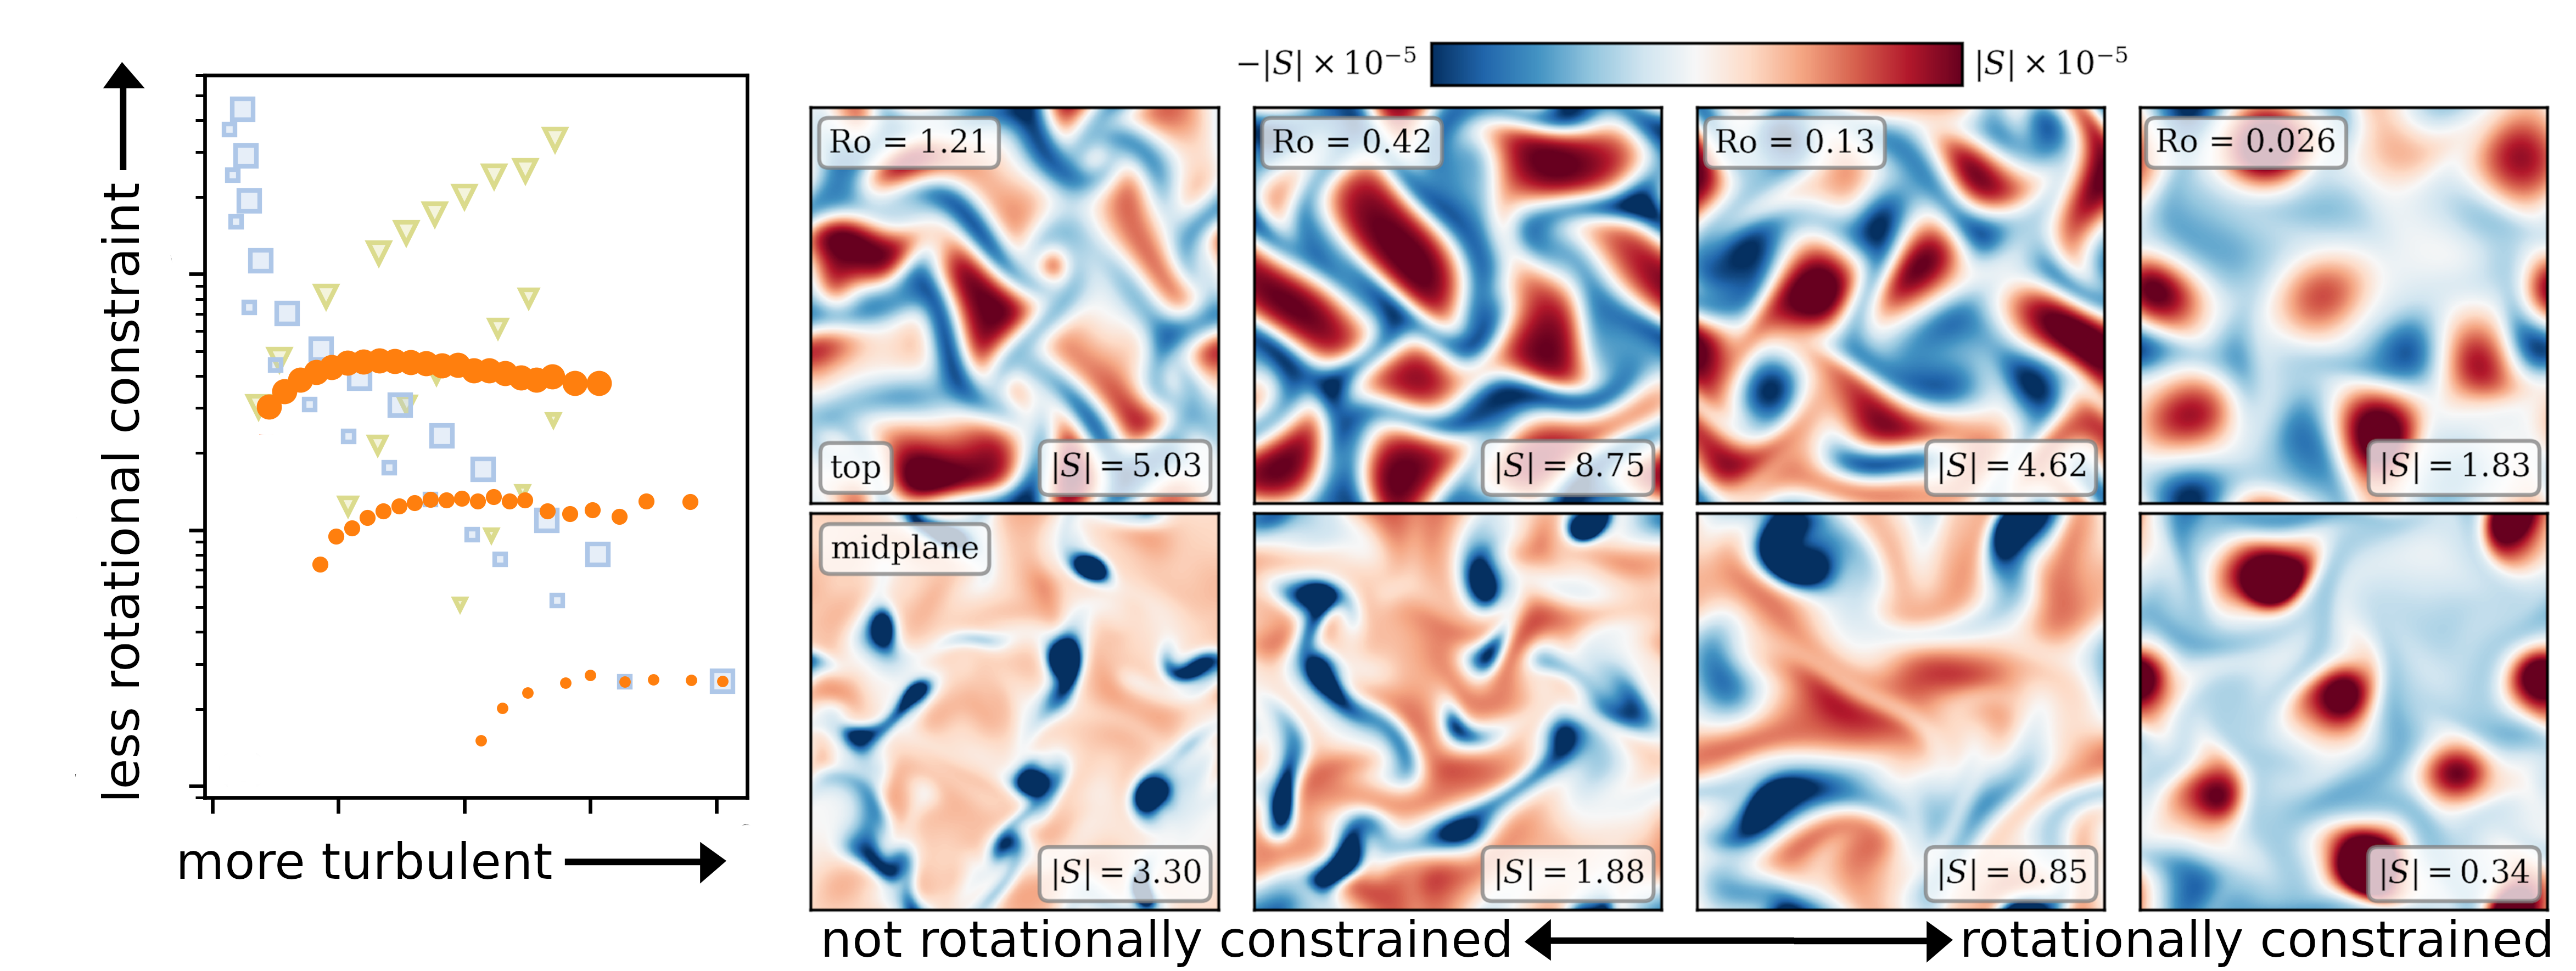
\includegraphics[width=\textwidth]{./figs/rossby_plot.png}
    \caption{(left, Fig 1b of \citet{anders&all2019}) The importance of rotation is difficult to predict as turbulence is increased in convective simulations.
	Rotational influence varies greatly along traditional paths through parameter space (green triangles and blue squares).
	We have discovered a new parameter (orange circles) that allows rotational influence to be specified \emph{a priori}.
	(right eight panels, Fig. 2 of \citet{anders&all2019}) As convective flows become increasingly rotationally constrained (from left to right), their morphology changes and they vary less as a function of height (top compared to bottom).
	It is crucial to simulate solar convection under the same rotational influence as the real Sun to ensure that flow topologies and interactions are an accurate model.
	\label{fig:rossby_plot} }
	\vspace{-6pt}
\end{figure*}

In creating simulations of solar convection, it is important to strive to produce flows which feel the same influence of rotation and magnetism as those in the Sun.
Simulations which include global rotation can be run in a regime where flows are heavily affected by Coriolis forces or one where Coriolis forces are weak.
A ``critical'' rotation frequency, $\Omega_\text{c}$, separates these two regimes, but determining $\Omega_\text{c}$ is often not straightforward.
During my PhD, I found a method for determining $\Omega_\text{c}$ so that the importance of rotation could be specified in simulation initial conditions \citep[see left panel of Fig. \ref{fig:rossby_plot} and][]{anders&all2019}.
Flows look very different depending on whether you simulate above, below, or near $\Omega_\text{c}$ (right panels of Fig.~\ref{fig:rossby_plot}), and it is crucial to simulate in the same regime as the Sun.
In magnetized systems, there is an analagous critical magnetic field, but to date no study has determined how to determine this field \emph{a priori}.

During my time at PCTS, I will study how an ensemble of downflows interacts with a solar-like RCB in the presence of solar-like rotation and magnetism.
In order to achieve this, I will first determine the critical magnetic field using similar techniques to those that I used during my graduate career while finding $\Omega_\text{c}$.
After determining this, I will study Cartesian simulations of localized, solar-like, rotating magnetoconvection and determine if downflows can effectively pump magnetic fields and angular velocity into a thin, solar-like RCB.
I look forward to collaborating with experts in astrophysical magnetohydrodynamics at Princeton and the IAS like Profs.~Eve Ostriker and Jim Stone on this project.

\vspace{-24pt}
\section{Global scale convection: dynamics in relaxed atmospheres}
\vspace{-8pt}
Modern 1D stellar models often employ the decades-old convective parameterization of mixing length theory \citep{bohm-vitense1958}, which has many deficiencies.
These deficiencies have led some researchers to seek out ways to couple 1D models with fully convective, three-dimensional (3D) global simulations.
Such a coupling has recently been performed with some success \citep{jorgensen&weiss2019}, but the 3D simulations utilized were localized in a very thin layer near the stellar surface.
Furthermore, \citet{jorgensen&weiss2019} coupled previously computed 3D simulations with 1D models, rather than coupling the two at runtime, largely because 3D simulations are costly.
Some of these costs are unavoidable: highly resolved, turbulent simulations necessarily take small timesteps, and therefore simulation times are very long.
Thin, near-surface simulations such as those used by \citet{jorgensen&weiss2019} examine a regime where the convective overturn timescale is very similar to the local Kelvin-Helmoltz (KH) timescale of atmospheric equilibration.
In studies of deep convection these timescales become disparate, and many overturn timescales pass during one KH timescale.
Thus, much of the expense of simulations which include deep convection is often time ``wasted'' waiting for the atmospheric structure and mean flows to converge to an equilibrium state.
This expense can be minimized through the use of clever numerical techniques.

\begin{wrapfigure}{r}{0.3\textwidth}
	\begin{center}
	\vspace{-10pt}
    \includegraphics[width=0.28\textwidth]{./figs/mdwarf.png}
	\vspace{-16pt}
	\end{center}
    \caption{A volume rendering of a global dynamo simulation in Dedalus.
	Enstrophy, or the magnitude of vorticity, is shown in green.
	Red and blue lines denote the magnitude and direction of azimuthal magnetic field.
	\label{fig:mdwarf} }
\end{wrapfigure}
During my PhD, I created and verified an ``accelerated evolution'' tool which skips the long KH timescale in convective simulations \citep{anders&all2018}.
This tool reached a relaxed, equilibrated state using an order of magnitude fewer computational resources than a simulation which timestepped through a full KH timescale, and results between the simulations differed by less than 1\%.

During my time at PCTS, I will extend my accelerated evolution method to the evolution of thermodynamic and angular momentum profiles in global simulations.
Dedalus is capable of accurately simulating global domains which include the origin at $r = 0$ \citep{lecoanet&all2019}; a visualization of basic outputs from these simulations is shown in Fig.~\ref{fig:mdwarf}.
The large-scale structures seen in Fig.~\ref{fig:mdwarf} arise quickly, but the equilibration and saturation of these structures and other simulation measurements often takes KH timescales which cannot be feasibly simulated in turbulent regimes.
I will design a generalized public module which can accelerate mean profiles and flows in global simulations.
This module will read in statistical measures from unequilibrated convective simulations and output the properly equilibrated mean state.
Researchers simulating convection with Dedalus or other codes will be able to use this module to rapidly equilibrate simulations with state-of-the-art turbulent dynamics.
This tool will benefit numericists across diverse research fields, such as those who study general circulation models (GCMs) in the atmospheres of the Earth and exoplanets or modelers of dynamo processes in planetary cores and stellar atmospheres.
Once completed, I will use this tool in my own research to accelerate the evolution of highly turbulent, solar-like simulations to understand the nature of global flows and dynamos in an equilibrated simulation.
I look forward to collaborating on this project with experts in global convective simulations like Princeton's Prof.~Adam Burrows as well as GFDL's many GCM experts.


\vspace{-24pt}
\section{Summary}
\vspace{-8pt}
The Princeton Center for Theoretical Science postdoctoral fellowship would give me the freedom to study these ambitious problems in astrophysical fluid dynamics.
The projects proposed here seek to understand stellar convection from small to global scales and build naturally upon my PhD research.
These projects help solve exciting problems in stellar structure with applications in numerous astrophysical subdisciplines.
Princeton is the perfect location for carrying out this work due to the opportunities available for interdisciplinary collaboration between astrophysicists, geophysical fluid dynamicists, and applied mathematicians.
I look forward to joining the center, creating cross-disciplinary collaborations, and carrying on Princeton's excellent research tradition while making lasting contributions which help solve the Convective Conundrum and other fascinating problems. 

\newpage
\bibliographystyle{apj_title}
\bibliography{biblio}
\end{document}
